\lhead{\emph{\leftmark}}  
\chapter{The Umplificator Technologies}
\label{chap:technology}
In this chapter, we provide an overview of the tool we have developed to support umplification; as well as discuss some of its technical details including its architecture and a detailed description of the Rule-Engine component. We also present the various design decisions we made as well as the alternatives implementations we attempted during the initial stages of our work. 

\section{The Umplification tool support goals}
In this section, we state what are the desirable aspects for a tool supporting the Umplification process. 

Our objective is to create an accurate tool that can enable developers to efficiently recover the model from existing software systems written in an object-oriented programming language. The Umplificator should provide extensible mechanisms to create and define transformation rules. In fact, the most important goal for a successful reverse engineering environment is that it must provide an extensible toolset \cite{tilley1994programmable}. The extensibility should be present in all the different operations of the tool such as parsing the input source code, transforming the source code and presenting the information. The end-user should be able to provide their own tools for these activities or to extend the ones already provided.  The high-level \textbf{general} and \textbf{specific} requirements for the tool are presented below. General requirements are the ones that every reverse engineering tool should possess and the specific requirements are the ones additionally required to implement the Umplification process (which may differ from other approaches).

\textbf{General Requirements}\\
A reverse engineering tool generally performs operations to gather information from a software system, organizes the information and presents it in manner such that software engineers can better understand the system. In the literature explored in Chapter \ref{chap:related} most of of the tools exhibit a layered architecture with a parser, analyzer and (XMI, XML) code generator as common components.

The general requirements for our specific tool are presented below with an emphasis on the component involved.

\begin{itemize}
\item The tool must be able to \textbf{parse} any of the most popular Object-oriented programming languages.
\item The tool must be able to handle of  the different idioms and programming conventions of those programming languages (parser and analyzer).
\item The tool should be able to \textbf{export} the output in Umple.
% When you say this it is not clear what formats you mean. You really mean Umple. What else?
% MG FIXED. Only Umple since Umple can then generate xmi, ecore...
\item The tool must offer both GUI and command-line capabilities. Command line capabilities are needed for automated testing, and scripting and for back-ends that permit deployment of the tool on the Web.
\item The tool should support incremental updates of the target model. This is required for large models as the target model does not need to be regenerated completely after each transformation. 
\end{itemize}

% Deleted a block here that was completely duplicated 
%MG -- FIXED

\textbf{From the developer's perspective:}
\begin{itemize}
\item The tool should be easy to debug. We should be able to quickly identify the location of an error and fix it.
\item The mapping rules should be as general and extensible as possible. 
\end{itemize}


\section{Alternative Approaches Studied}
We have explored two different and famous model transformation technologies with the purpose of umplifying a software system: TXL \cite{Cordy2006} and ATL \cite{atl}. In the following two sub-sections we present the mapping rules, grammar and program directives that allowed us to transform a Java Program into Umple. 

\subsection{TXL}

TXL is "a programming and rule-based language and rapid prototype system designed for implementing source transformation tasks" \cite{Cordy2006}.

The TXL paradigm consists of parsing the input text into a tree according to a specified grammar, transforming the tree to create a new output parse tree and processing the new tree to finally produce the output text. In TXL, grammars and transformation rules are specified in the TXL programming language. The TXL processor is responsible for interpreting both the grammar and mapping rules by using an internal tree-structured bytecode. TXL programs depend on no other tools or technologies and can run on any platform directly from the command line.

TXL programs are composed of a\textit{ base grammar}, which specifies the syntactic forms of the input structure, a set of \textit{grammar overrides}, which extend the grammar to be used and a set of \textit{transformation rules and functions}, that specify how the input structure will be transformed to produce the desire output structure.

The \textit{grammar} in TXL is a set of recursive rewriting rules used to generate patterns of strings. A grammar in TXL is used to specify how the input is partitioned into tokens of the input language and how the sequences of input tokens are grouped into structured types of the program. 

The\textit{mapping rules and functions} specify how to transform the input text into the desired output. The mapping rules are specified using pattern and replacement pairs: 

\vspace{\baselineskip}
\begin{lstlisting}[style=umplePlain]
LeftHSPattern -> RightHSPattern IF Condition
\end{lstlisting}

Where \textit{LeftHSPattern} and \textit{RightHSPattern} are term patterns. The result of a mapping rule is the instantiation of the \textit{RightHSPattern} and is produced when the term matches the \textit{LeftHS\_Pattern} and the condition is true. Rules are applied recursively until they fail. Functions are similar to Rules but they are applied once on the entire function input.

TXL has been used widely in software engineering tasks and other areas including database migrations and artificial intelligence. We present our experiment in building a \textit{Java-to-Umple} transformer using TXL. We first studied the similarities and differences between Java and Umple and classified the necessary transformations for converting Java programs to Umple into three categories.

The first category represents the direct transformations where one-to-one mapping between the two languages exists and some rules for minor adaptations are required. For instance, a Java class declaration can be written as: 

\vspace{\baselineskip}
\begin{lstlisting}[style=umplePlain]
ClassModifier class Identifier TypeParameter Super Interfaces ClassBody
\end{lstlisting}

In this, the \textit{ClassModifiers} are used to control the access to members of a class, the Identifier specifies the name of a class, the optional \textit{TypeParameter} are used when the class is generic and declares one or more type variables, the Super clause specifies the direct superclasses of the current class, and the Interfaces clause specifies the name of the interfaces that are direct super-interfaces of the class being declared.

Very similarly, an Umple class is defined as: class Identifier \textit{ClassBody}. In this case we will need a mapping rule matching the Identifier and class keyword in the Java program to produce the desired output, the Umple class. 

The second category corresponds to the \textit{indirect transformations} where some special functions are needed to map a Java construct to an Umple one. For example, a Java instance variable can be mapped to an Umple attribute, an Umple Association or an Umple state machine. This kind of transformations requires helper and additional functions in the TXL program. 

\subsubsection{Java to Umple Implementation}

In this section, we describe the design process. Next, we describe the implementation of the \textit{JavaToUmple} program that partially converts Java code to Umple. Lastly, we provide examples of transformations rules in the TXL language. Figure \ref{fig:txl} presents the components of the TXL \textit{JavaToUmple} program. 

\begin{figure}[h]
\centering
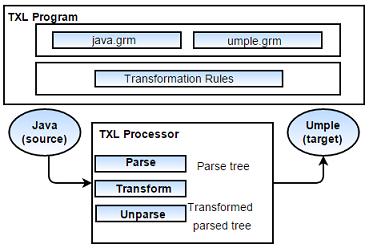
\includegraphics[width=0.75\textwidth]{Figures/TXLprogram.png} 
\caption{TXL Program for transforming Java to Umple}
\label{fig:txl}
\end{figure}

\subsubsection{Design process of the TXL Program}

The first step in writing a source transformer is writing working grammars for both the target and the source language and then writing a union grammar that accepts constructs for both languages. A grammar for Java 1.5 is available from the TXL website \cite{txlresources}. We wrote the grammar for Umple in EBNF format required by the transformation engine. We then built the TXL rules and functions grouped in modules. Each module targets conversion of one specific language construct of Java to the equivalent in Umple and is stored in a separate file. The overall structure of the transformer is shown in Figure \ref{fig:txlStructure}. It contains the modules for the different language constructs and the main program that starts the program. Below, we briefly describe the different modules:

\begin{figure}[h]
\centering
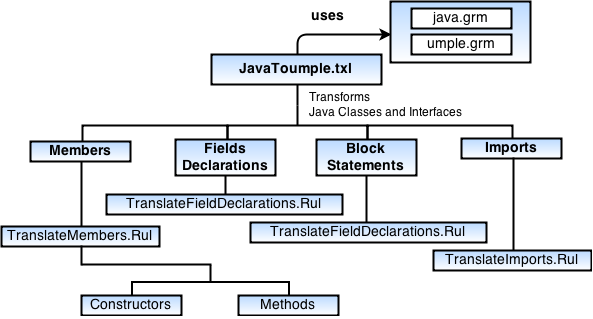
\includegraphics[width=0.98\textwidth]{Figures/TXL_STRUCTURE.png} 
\caption{Structure of the JavaToUmple program}
\label{fig:txlStructure}
\end{figure}

\begin{itemize}
\item JavaToUmple.Txl: This is the main program. It is used by TXL to match an input Java program against the Java Grammar and to call the transformation rules.
\item TranslateMembers.Rul: Contains rules and functions to transform nested declarations.
\item TranslateFieldDeclarations.Rul: Contains rules and functions to transform field declarations.
\item  TranslateBlockStatements.Rul: Contains rules and functions for matching bodies of code belonging to constructors and methods.
\item TranslateImports.Rul: Contains rules for matching Java imports.
\item TranslateConstructors.Rul: transforms the Java constructors.
\item TranslateMethods.Rul: transforms Java Methods.
\end{itemize}

The original Java source code remains untouched after applying the transformation. A set of one or more Umple files is produced as a result of the transformation. The \textbf{JavaToUmple} program can be invoked using the command:

\vspace{\baselineskip}
\begin{lstlisting}[style=umplePlain]
< txl –o outputFileName.ump inputFileName.Java JavaToUmple.txl >
\end{lstlisting}

In the following sub-section we provide some transformation examples. We first show the Java and Umple grammar for the single constructs we transform as well as the TXL transformations rules that guide the transformation.

\subsubsection{Transformation 1: Transforming the Class Header} 

In order to transform a Java class into an Umple class, we need to first transform the class header. The code excerpt in Listing \ref{lst:bnftxl} below shows the EBNF grammar for class definitions in both Java and Umple languages. An example of class definitions is also provided in Listing \ref{lst:sampletxl}.

\begin{lstlisting}[style=umplePlain, caption="Class definition grammar in BNF form", label=lst:bnftxl]
JavaClassDeclaration: 
   ClassModifiers? class Identifier Super? Interfaces? ClassBody


UmpleClassDeclaration: 
   class Identifier ClassBody  ClassBody: '{' ClassContents '}'

\end{lstlisting}

\begin{lstlisting}[style=umplePlain, caption=Class definitions in Java and Umple, label=lst:sampletxl]
// In Java:
public class A extends X implements Z {
    //…some contentW
}
// In Umple:
class A 
{	
 //.. some content
}
\end{lstlisting}

The mapping rule called `\textit{changeClassHeader}' in file \textit{TranslateMembers.Rul} that transforms class headers of a Java class is presented below in Listing \ref{lst:classHeader}. In order to transform the class header from Java to Umple, we need to deconstruct the class header  (Line 4)  of a Java class and take only what is required in an Umple header, the identifier of the class. The modifiers of the class are discarded and the extends and implements clauses are ignored at this moment, they are analyzed and transformed in subsequent steps of the program transformation. 

\begin{lstlisting}[style=umplePlain, caption=TXL Mapping rule for transforming the class headers, label=lst:classHeader]
rule  changeClassHeader 	
   replace $[class_header] 		
    	ClassHead[class_header] 		
    	deconstruct ClassHead 					
    	modifiers[repeat modifier] 'class Name[class_name] 
        ExtendClause[opt extends_clause] 
        ImplmntClause[opt implements_clause]          
    by 	 'class Name 
end rule

\end{lstlisting}

\subsubsection{Transformation 2: Transforming the package} 

A \textbf{package} in Java can be defined as a grouping of related classes (and types). In Umple a \textbf{namespace} allows to group Umple classes. Listings \ref{lst:txlpackage} and \ref{lst:txlpackage2} show the EBNF grammar of package definition in both languages and an example. 

\noindent\begin{minipage}{.45\textwidth}
\begin{lstlisting}[style=umplePlain,caption=Java Package,label=lst:txlpackage]{Name}
PackageDeclaration:
   package PackageName; 

package aPackageName;
\end{lstlisting}
\end{minipage}\hfill
\begin{minipage}{.45\textwidth}
\begin{lstlisting}[style=umplePlain,caption=Umple Namespace,label=lst:txlpackage2]{Name}
PackageDeclaration:
   namespace NamespaceName;
 
namespace aNamespaceName;
\end{lstlisting}
\end{minipage}


The mapping rule called `\textit{changePackageToNamespace}' that transforms package declarations is presented below:

\begin{lstlisting}[style=umplePlain, label=lst:packageDeclRule3, caption=TXL mapping rule for the transformation of the package declaration]
rule changePackageToNamespace 
    replace [opt package_header]      
            'package Name [package_name] '; 
    by       
            'namespace Name '; 
end rule	
\end{lstlisting}

\subsubsection{Transformation 3: Transforming the imports} 

An import declaration in Java allows a named type or a group of named types to be referred to. The `\textit{Depends}' construct in Umple is similar to this. 

\noindent\begin{minipage}{.45\textwidth}
\begin{lstlisting}[style=umplePlain,caption=Java Import]{Name}
ImportDeclaration:
     import  QualifiedName; 


import java.io.StreamReader;
public class A {
 //…
}
\end{lstlisting}
\end{minipage}\hfill
\begin{minipage}{.45\textwidth}
\begin{lstlisting}[style=umplePlain,caption=Umple Depend]{Name}
DependDeclaration:
   depend QualifiedName;


class A {
  depend java.io.StreamReader;
}
\end{lstlisting}
\end{minipage}

The mapping rule called `\textit{changeImportToDepend}' in file \textit{TranslateImports.Rul} that transforms import declarations is presented below: 

\begin{lstlisting}[style=umplePlain, label=lst:packageDeclRule, caption=TXL mapping rule for the transformation of the import declaration] 
changeImportToDepend  	
    replace [repeat import_declaration]      
           'import Name [imported_name] '; 
    by 	   'depend Name '; 
end rule
\end{lstlisting}

As seen in the example, the depend declarations appear inside the Umple class, so we need additional rules to remove them from the top of the Java class and place them in the right place prior the generation of the Umple code. The rule below removes all the import declarations. The main program, presented next, illustrates how the program executes the mapping rules in order to produce the output. Note that in TXL the input program is not modified since the transformation only occurs on the parse tree of the input program.

\begin{lstlisting}[style=umplePlain, label=lst:packageDeclRule2, caption=Helper Function used to remove the imports declarations] 
function removeImports  
    replace * [package_declaration]
        PkgHead [opt package_header]   
        ImpDecl [repeat import_declaration]  
        TypeDecl [repeat type_declaration] 
    by   
        PkgHead      TypeDecl
end function
\end{lstlisting}


\subsubsection{Final transformation: The main program}

The main program in Listing \ref{lst:mainProgramtxl} is used to execute the three mapping rules presented in the examples above; it calls one by one the rules and the functions and generates the output. Additionally, the main program links, via inclusion constructs, the grammars from the target and source languages (Line 1-2). In the \textbf{JavaToUmple} program we use two grammar files to map Java and Umple constructs: \textit{Java.GRM} and\textit{ Umple.GRM}.

\begin{lstlisting}[style=umplePlain, label=lst:mainProgramtxl, caption=The ATL main program - JavaToUmple.Txl] 
include "java.Grm" 
include "Umple.Grm" 

function main    
    replace [program]
        P [program]     
    by 	P [javaToUmple]
end function 

function javaToUmple   
    replace [program] 
         P [program]     
    by 
        P 
        [changePackageToNamespace] 
        [changeImportToDepend] 
        [removeImports] 
        [changeClassHeader]
end function 
% ****	MAPPING RULES HERE   ****
\end{lstlisting}

The transformation program above uses the two grammar files to map Java and Umple constructs:  java.GRM and Umple.GRM. The program rules have been modularized for a better understanding as has been shown in Figure \ref{fig:txlStructure}.

\subsection{ATL}

ATL (ATL Transformation Language) \cite{atl} is a model transformation language that provides ways to produce a set of target models from a set of source models and allows users to define model-to-model transformations in both a declarative and imperative way.

ATL has been developed in Eclipse as a set of plug-ins by the Institut National de Recherche en Informatique et en Automatique (INRIA) as an answer to the Object Management Group's QVT language request for proposals \cite{Jouault200831}.  The ATL environment in Eclipse offers an ATL editor with syntax highlighting and code completion capabilities, a debugger and a profiler that aims to ease the development and testing of model transformations.

In this section, we describe how queries, views and transformations are handled in ATL. Additionally, we explore the ATL transformations required to umplify a Java system. Figure \ref{fig:atl} presents the necessary components to implement and ATL transformation between Java and Umple. An ATL program (\textit{JavaToUmple.atl} in the Figure) takes model \textit{Java.xmi} as input and produces model \textit{Umple.xmi} as output. Both models need to be expressed in the OMG XMI standard \cite{xmispec}. The Java model conforms to metamodel \textit{Java.ecore} and the Umple model to metamodel \textit{Umple.ecore}. The ecore \cite{ecore} notation is a simple metamodel specification language. The ATL program \textit{JavaToUmple.atl} is also a model, so it conforms to a metamodel (the ATL metamodel). As we will see in Section \ref{subsubsec:exampleATL}, the program is composed of a header, a set of helper functions and a set of (transformation) rules.

\begin{figure}[h]
\centering
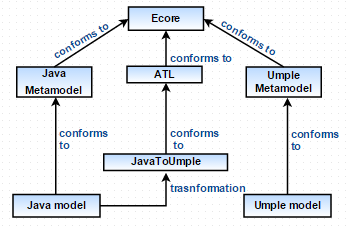
\includegraphics[width=0.75\textwidth]{Figures/ATL_PROGRAM.png} 
\caption{The JavaToUmple ATL program}
\label{fig:atl}
\end{figure}


\subsubsection{The basics of ATL}

The ATL language is composed of expressions to query model elements (queries), views to handle incremental transformations and transformation rules to direct the transformations of  a set of source models to a set of target models.

\textbf{Queries}

A query in ATL is an expression allowing one to search and return model elements from a model defined in an OMG-compliant format. A query is an OCL expression that can return primitive values, model elements or a combination of these. A query can not alter the source model. It is possible to navigate across model elements and call query operations on these. For instance, when the following query is executed on a Java model, it first gets the set of all existing JavaElement classes in the model and gets the size of the computed set. The computed integer value is cast into a string before being written into the file `metrics.txt'. 

\vspace{\baselineskip}
\begin{lstlisting}[style=umplePlain]
query JavaElementNb  =
  JavaModel!JavaElement.allInstances()->size().toString()
       .writeTo('metrics.txt')
\end{lstlisting}


\textbf{View}
Views in the ATL world are a special case of transformation. Views offer support for incremental transformations. The user can query a model; perform a transformation on a subset of the source model and save results on a view. Then, she can update the view from its source without executing the whole transformation again. 

\textbf{Transformation Rules}
There are different kinds of rules in ATL based on the way they are called and how they specify the results: matched rules, lazy rules and called rules \cite{stephan2009comparative}.

\begin{itemize}
\item \textbf{Matched Rules}: 	This kind of rule specifies which source element is to be matched, along with the target element that is to be produced.

\item \textbf{Lazy Rules}: This kind of rule is similar to a matched rule, but it is not executed when matched; they rely on being called by other rules.

\item \textbf{Called Rules:}	This kind of rule can have parameters and can be called only from blocks of imperative code. Assignments, `for' and `if' statements are the only three types of (imperative) statements supported in ATL.

\end{itemize}

\subsubsection{ATL Tool Support \textemdash Eclipse M2M}
%The long-dash above doesn't appear in the output
% MG Fixed
The ATL project is composed of four parts (or four different plug-ins in Eclipse). The Core, Compiler, Parser and the Virtual Machine (VM) \cite{Jouault200831}, which are described below:

\begin{itemize}
\item \textbf{Core} - Contains the classes used to internally represent a model, to allow the creation of models and metamodels, to save and load models and to supply ways to launch the model transformations. 
\item \textbf{Compiler} - Uses the ACG (ATL VM code generator) domain-specific language to compile and generate code. 
\item \textbf{Parser} -Contains all classes to parse an ATL transformation input and to generate an output model compliant with the target metamodel.
\item \textbf{VM} - A byte-code interpreter.
\end{itemize}

\subsubsection{Transformations Examples with ATL}
\label{subsubsec:exampleATL}

In this section we provide some transformation examples in ATL. We present parts of the metamodels, models, mapping rules and the final results (Umple code) of some Java to Umple ATL model transformations.
The JavaModel to UmpleModel examples describe a transformation from a simplified Java Model to an Umple model. 

\textbf{Metamodels} 

The source metamodel of Java in Figure \ref{fig:javamodelatl} consists principally of \textit{JavaElements} which all have a name. A \textit{JavaClass} has Methods and Fields and belongs to a package. \textit{Methods}, \textit{Fields} and \textit{JavaClasses} are subclasses of the class Modifier and indicate whether they are public, static or final. Java classes and methods declare with the isAbstract attribute whether they are abstract or not. Fields and methods have also a Type. The Java metamodel in Figure 6 has been fully described by the Java Specification \cite{javaSpec} and has been simplified for the purpose of this transformation example.

\begin{figure}[h!]
\centering
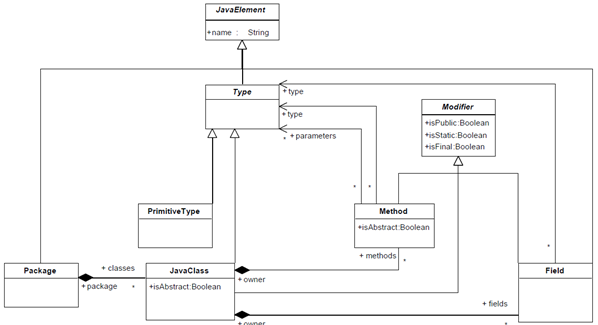
\includegraphics[width=0.99\textwidth]{Figures/javametamodel.png} 
\caption{A simplified version of the Java metamodel}
\label{fig:javamodelatl}
\end{figure}

\begin{figure}[h!]
\centering
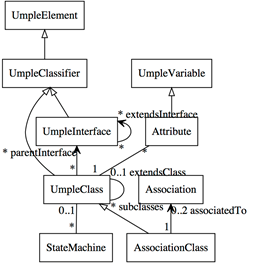
\includegraphics[width=0.55\textwidth]{Figures/umpleMetamodel.png} 
\caption{A simplified version of the Umple metamodel}
\label{fig:umplemodelatl}
\end{figure}
A simplified version of the Umple metamodel (target metamodel) is presented in Figure \ref{fig:umplemodelatl}. The complete metamodel for Umple can be found at \cite{UmpleMetamodel}. Both metamodels have been defined in XMI format, as required by the ATL metamodel loader.

\paragraph{Transformation rules} 

These are the rules to transform a Java Model to an Umple model. The ATL code for the transformation, shown in Listing \ref{lst:atlrules} consists of several functions and rules. Among the functions, we can mention the \textit{getExtendedName} in Lines 4-8 which recursively explores the namespace to concatenate a full path name.

%The following listing results in the caption at the bottom of a page, a figure injected, and then the listing itself. Is it possible to force the caption to always stick to the rest of the listing (i.e. 'keep with next' in Word)
% MG Fixed.

\begin{lstlisting}[style=atl, label=lst:atlrules, caption=ATL Transformations rules]
module JavaToUmple;
create OUT: Umple from IN: Java;

helper context Java!Namespace def: getExtendedName() : String = 
	if self.namespace.oclIsUndefined() then '' 	
	else if self.namespace.oclIsKindOf(UML!JavaModel) then 	'' 
	else self.namespace.getExtendedName() + '.'
endif endif + self.name;

rule P2P { 
	from j :Java!Package (e.oclIsTypeOf(Java!Package)) 	
	to out : Umple!Namespace ( 		
			  name <- j.getExtendedName())
}

rule C2C { 	
	from j : Java!JavaClass 	
	to out : Umple!UmpleClass ( 	
			name <- j.name, 	
			isAbstract <- j.isAbstract,      
			// .. parts ignored		
	)
}

rule F2A { 	
	from j : Java!Field to out : Umple!UmpleAttribute ( 		
	name <- j.name,
	value <-  FieldHelper.getValue(j) 	
	isConstant <- FieldHelper.isContant(j), 		
	isImmutable <- FieldHelper.isImmutable(j), 		
	isLazy <- FieldHelper.isLazy(j),
	)
}

\end{lstlisting}

% In Latex you have to use quotes like this `quoted' and ``double''. I fixed some cases in the next paragraph. You will want to search the thesis for more.

The three rules presented above are part of the set of rules required to transform a Java Model to an Umple model.  The first rule `\textit{P2P}' in Lines 10-14  specifies how to map a Java package to an Umple namespace. The second rule `\textit{C2C}' in Lines 16-23 declares how we can match a Java Class to an Umple Class. The last rule `\textit{F2A}' aims at transforming a Java Field to an Umple Attribute. This rule is a \textit{called rule} as it is just called whenever a Java Field matches an Umple Attribute. Remember that a Java Field can match an Attribute, Association or State Machine in Umple.

The \textit{FieldHelper} (Lines 29-33) used in rule \textit{F2A} is an utility class used to determine certain properties of a Java field that can derive into properties of a Umple attribute. For instance the \textit{FieldHelper.isLazy(aJavaField)} returns \textit{true} if the java field passed as parameter is not one of the constructor parameters of its parent class. This helper class is also used to compute components of a Java Field not having a one-to-one match to an Umple class. The (static) method \textit{FieldHelper.getValue(aJavaField)} extracts the value of a field (if any). 

\section{Discussion}

% I think here you ought to discuss the CDT approach (at least give the sort of background you gave for TXL and ATL) without explaining in detail how you used it.

% Here you need to explain the issues you had with TXL and ATL.This should be at least two pages. There should be a table showing comparisons between TXL, ATL and CDT, and a conclusion about why you chose the latter. Stopping for the day.

\section{The Umplificator}
\label{chap:tool}
In this section, we provide a detailed description of the tool we have developed to support umplification; as well as discuss some of its technical details.

Our tool called, Umplificator, takes as input  a set of files containing classes written in base language code (Java, C++ etc.), Umple files, source code directories or software projects (source code containers as represented in many popular IDEs such as Eclipse). The output is an Umple textual model containing base language code with modeling abstractions. 

%DELETE The Umple model is fully compatible with many UML and XMI formats and can be viewed or edited diagrammatically. 
%I suggest deleting this. I assume you have a decent discussion of Umple earlier.
% MG Yes, fine by me.

At its core, the Umplificator is a language interpreter and static analyzer that parses base language and Umple code/models, populates a concrete syntax graph of the code/model in memory (\textit{JavaModel}, \textit{CPPModel}), performs model transformation on the base language representation in memory and then outputs Umple textual models.

The Umplificator relies on initial parsing by tools such as the Java Development Tool (JDT) for Java, CDT for C++, and PDT for PHP. These extract the input model from base language code. The use of JDT and its siblings reduces the need to write an intermediate parser for the base language.

The base language model is then transformed in a series of steps into an Umple model. To do this, the Umplificator uses a predefined set of refactoring rules written in the Drools rule language \cite{Drools_Book}. Drools is a rule management system with a forward- and backward-chaining rules engine. 

% MG FIXED
%REally 4.2? I assume this is supposed to be a forward reference. If in fact you have already discussed it, then don't introduce it again in the above paragraph.
The Umplificator includes other subsidiary and internal tools such as:
\begin{itemize}
\item Language validators – A set of base language validators allowing validation of the base language code that is generated after compilation of the recovered Umple models.
\item Umplificator statistics –  A metrics-gathering tool to analyze certain aspects of a software system such as the number of classes and interfaces, the  number of variables present in the code, the cyclomatic complexity, the number of lines of code \cite{MetricsBuse}.  
\item Umplificator Workflow – A tool that guides the umplification process within Eclipse.
\end{itemize}

The development of the Umplificator follows a test-driven approach to provide confidence that future enhancements will not regress previously functioning and tested aspect of the system. Test-driven testing for the Umplificator is discussed in section \ref{sec:testingUmplificator}. 

\subsection{Architecture}
\label{sec:architecture}

The Umplificator has a layered and pipelined software architecture. The pipelines (components) in this architectural style are arranged so that the output of each element is the input of the next.  Figure \ref{fig:architecture} presents the architecture which is comprised  of four components. The parser, model extractor, transformer and generator components are explained in the following sub-sections.

The process of umplifying am object-oriented software system in this architecture is described below an illustrated in Figure \ref{fig:process_flow}.

\begin{enumerate}
\item  The input is a set of source code files in the base language and/or Umple.
\item (Parser) The source code is parsed. 
\item (Model Transformer) The source code is transformed into base-a model of the base language and Umple constructs.
\item (Transformer) The model previously obtained is entered into the next stage of the pipeline. The input model is transformed a model with additional Umple features using pre-defined mapping rules. 
\item The target Umple model, is then validated. 
\item (Generator)Finally, Umple code (.ump files) are generated from the Umple model.
\end{enumerate}

\begin{figure}[h]
\centering
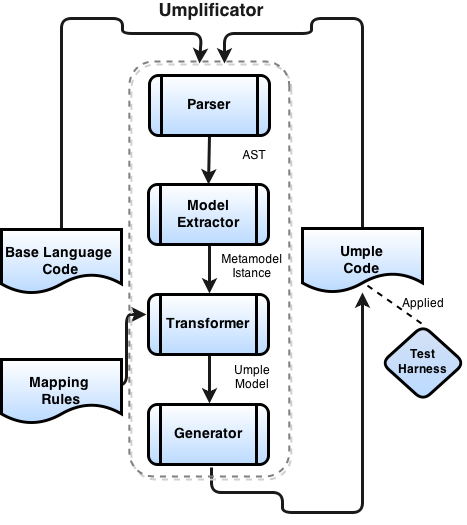
\includegraphics[width=0.75\textwidth]{Figures/Umplificator_ProcessFlow.png} 
\caption{The umplification process flow}
\label{fig:process_flow}
\end{figure}

The Umplificator employs the libraries and technologies summarized in Table \ref{table:technologies} to implement its reverse engineering capabilities. The dependencies between the external and internal components of the Umplificator is shown in Figure \ref{fig:architecture}, where our \textit{Parser} and \textit{ModelExtractor} components uses the JDT/CDT/PDT projects and the \textit{Transformer} the Drools Rule Engine. 

\begin{figure}[h]
\centering
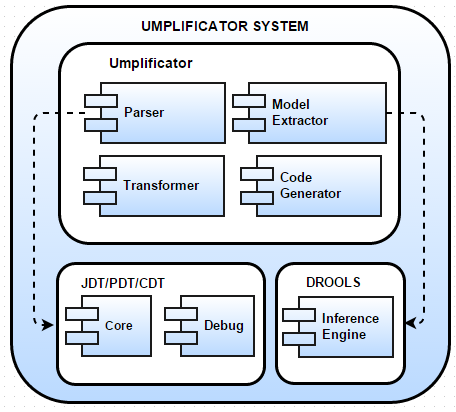
\includegraphics[width=0.75\textwidth]{Figures/UmplificatorComponents.png} 
\caption{The Umplificator components}
\label{fig:architecture}
\end{figure}

% Make the above figure's text a little smaller and less bold to make it look nicer.
% MG Fixed
The Table also shows the Umplificator component using the technology. Note that if the technology is used in more than one component, we mark it as `General'.

\begin{table}[h]
\caption{Third Party Technologies employed in the Umplificator tool}
\label{table:technologies}
\begin{tabularx}{\textwidth}{l|YY}
\toprule
\rowcolor[HTML]{BBDAFF}
\textbf{Technology} & \textbf{Targeted component(s)}  & \textbf{Description}  \\ \hline
JDT/CDT/PDT  & Parser and Model Extractor & APIs for parsing object-oriented source code.\\ \hline 
Drools Rule Engine & Transformer  & A Rule Engine for creating and managing the mapping rules used in the Umplificator.	 \\ \hline	
JOpt Simple & General  & Library for parsing command line options \\ \hline	
Log4j & General & A logging library used to collect (reverse-engineering) process data.	\\ \hline	
Perf4j & General & Set of utilities for calculating and displaying performance statistics in the Umplificator code. \\ \hline	
\end{tabularx}
\end{table}

The different components of the Umplificator as well as the third-party technologies employed are discussed next. 

\subsection{Parser and Model Extractor}

The parser component receives a set of source code files in the base language and/or Umple and creates an abstract syntax tree (AST) as representation of the code. Umple code is allowed as input to allow repeated application to refine the model. To implement its parsing and base language model extraction capabilities, the Umplificator uses various Eclipse Projects, as summarized in the following table. These projects provide APIs to access and manipulate object-oriented source code.
They also provide access to the  source code via two different means: a base language model within the Eclipse Workspace and an Abstract Syntax Tree (AST) for a standalone usage (outside the Eclipse IDE). Table \ref{table:xdtProjects} summarizes the Eclipse projects used in the Umplificator for \textbf{parsing} purposes. We then provide some details about the capabilities and usage of each project. 

\begin{table}[h]
\caption{Eclipse projects used in the Umplificator}
\label{table:xdtProjects}
\begin{tabularx}{\textwidth}{l|YY}
\toprule
\rowcolor[HTML]{BBDAFF}
\textbf{Project} & \textbf{Targeted programming language}  & \textbf{Components used (plug--ins)}  \\ \hline
	Java Development Tooling & Java   & org.eclipse.jdt.core , org.eclipse.jdt.core.dom  \\ \hline
	C++ Development Tooling  & C++   & org.eclipse.cdt.core \\ \hline
	PHP Development Tools	 & PHP   & org.eclipse.pdt.core \\ \hline
\end{tabularx}
\end{table}

Eclipse is not simply a programming language IDE. In fact,  Eclipse is an extensible platform for building IDEs. Eclipse functionality is wrapped into pluggable components called \textit{plug-ins}. These plug-ins allow developers to extend the basic functionality offered by Eclipse. The projects mentioned in the above table, are plug-ins that can be used in other projects inside Eclipse or as a standalone component, as in our case.

Architecturally, the JDT/CDT/PDT projects are divided into two domains: the model (core) and the user interface. The model is a representation of the Base language elements; the user interface is a set of views, actions, perspectives and menus that work together. The user interface domain can be extended but only works inside Eclipse (not intended for standalone usage).  The Umplificator uses the model component of these projects to \textit{parse} and \textit{extract} a base language model from source code. 

\textbf{Java Development Tooling (JDT)}

 Eclipse Java Development Tooling (JDT) \cite{jdtProject} offers a comprehensive Java development environment. JDT also provides APIs for analyzing Java source code. It provides several levels of source code analysis that can be reused. The level of source code analysis used in the Umplificator is the Abstract Syntax Tree (AST) framework. We use the AST to analyze the Java source code as a tree of nodes, where each node represents a part of the source code (for instance a variable declaration, a method body, a contructor and so on). The AST framework defines over 60 \textit{ASTNode} \cite{astnodeapi} subclasses representing the different elements of the Java language. 
 
% I dpn't get 'over ASTNODE' above
% MG. Over 60 subclasses...
  
The AST framework includes also interfaces that help retrieve specific source information beyond what is indicated by the ASTNode source pointers. To traverse the nodes returned by the parser (ASTParser) and collect the desired information about the source code, we employ multiple visitor classes that follows the Visitor software design pattern \cite{gamma1994design}. 
The visitor pattern is a standard way to decouple the data from the operations that process the data.
For each different AST node type T, two methods are offered:

\begin{itemize}

\item  \textit{public boolean visit(T node)} -- Visits the given node to perform some arbitrary operation. If true is returned, the given node's child nodes will be visited next;
\item  \textit{public void endVisit(T node)} --  This method is called after all of the given node's children have been visited (or immediately, if visit returned false). The default implementation provided by this class does nothing;
\end{itemize}

Generally, the AST visitor can be used to \textbf{transform} AST nodes or to \textbf{derive} information. A derivation collects information and stores result along the way. For instance, if our intention is just to collect the import declarations of a Java class, we could write a visitor as in Listing \ref{lst:importvisitor}. In the method visit(...) we return false to stop the visitor from visiting child nodes of the import declaration. The variable \textit{importDeclarations} is an array containing the (visited) import declarations. 

\begin{lstlisting}[style=java, caption=A visitor for Import declarations in Java source code, label=lst:importvisitor]

public class SimpleVisitor extends ASTVisitor{

	private List<ImportDeclaration> importDeclarations;

	public boolean visit(ImportDeclaration node) {
	    importDeclarations.add(node);
	    return false;
	}
}
\end{lstlisting}

As an example, consider the code of class `\textit{Test}' in Listing \ref{lst:astjava}. Once the code is parsed, we used a visitor to collect the desired information. Table \ref{table:astanalysis} presents the resulting AST node types, the corresponding source fragment and the visitor employed to collect the information. This Table recapitulates the entire process of parsing and extracting the model for our sample code. 


\begin{lstlisting}[style=java, caption=Test.java, label=lst:astjava]
package umplificatorTest;

import java.util.Date;

public class Test {
	public int number;
	
	public int  getNumber() {
		return number;
	}
}
\end{lstlisting}

\newcommand*{\MyIndent}{\hspace*{0.4cm}}%
\begin{table}[h]
\caption{Sample Uses of an AST for Code Analysis}
\label{table:astanalysis}
\begin{tabularx}{\textwidth}{l|YY}
\toprule
\rowcolor[HTML]{BBDAFF}
\textbf{ASTNode Type} & \textbf{Source Fragment}  & \textbf{Visitor Code}  \\ \hline	
\textbf{CompilationUnit} &  Entire source code & visit(CompilationUnit cu) \\ \hline
\MyIndent \textbf{PackageDeclaration} & "package umplificatorTest" & visit(PackageDeclaration pd) \\ \hline
\MyIndent \textbf{TypeDeclaration} &  "public class Test" & visit(TypeDeclaration td) \\ \hline
\MyIndent \MyIndent \textbf{FieldDeclaration} &  "public String name" & visit(FieldDeclaration fd) \\ 
\MyIndent \MyIndent \MyIndent PrimitiveType("int") &   & \MyIndent td.getType() \\ 
\MyIndent \MyIndent \MyIndent SimpleName("number") &   & \MyIndent td.getSimpleName() \\ \hline
\MyIndent \MyIndent \textbf{MethodDeclaration} &  "public int getNumber()" & visit(MethodDeclaration md) \\ 
\MyIndent \MyIndent \MyIndent PrimitiveType("int") &   & \MyIndent td.getReturnType() \\ 
\MyIndent \MyIndent \MyIndent SimpleName("getNumber") &   & \MyIndent td.getName() \\ \hline
\MyIndent \MyIndent \MyIndent \MyIndent \textbf{Block} & "{..}"& \MyIndent bl=  md.getBody() \\ 
\MyIndent \MyIndent \MyIndent  \MyIndent \MyIndent \textbf{ReturnStatement} &  "return number;" & stmt = b1.getStatements(0); \\ \hline
\end{tabularx}
\end{table}

Note that the AST node type CompilationUnit is the type root of an AST (first row of above table) and the object returned by the ASTParser after completion of the parsing a Java file. The source range for the CompilationUnit type node is the entire source file, including leading and trailing whitespace and comments. In Java 1.4 to 1.7, a CompilationUnit is composed of 
a \textit{PackageDeclaration}, \textit{ImportDeclaration}, and one or more of these types:  \textit{TypeDeclaration}, \textit{EnumDeclaration}, \textit{AnnotationTypeDeclaration}. 

The code on the right of Table \ref{table:astanalysis} shows several examples of what can be done inside a visitor method:

% change the phrasing below to avoid the second person 'you'. i.e. get rid of 'Do you 
% MG FIXED
\begin{itemize}
\item Extracting the name of the package: Code a \textit{visit(PackageDeclaration)} and get its name as an instance of \textit{SimpleName} (e.g. package test)  or \textit{QualifiedName} (e.g. package cruise.compiler.*).
\item Getting the list of types referenced in a compilation unit? Code a \textit{visit(TypeDeclaration)} and get theirs names as instances of \textit{Simple} or \textit{QualifiedName}.
\item Finding all literal integers referenced only within methods and not fields? Code a `sub' \textit{visit(IntegerLiteral)} inside the visit method for \textit{MethodDeclaration}.
\end{itemize}

\textbf{Java Development Tooling (CDT)}

In the same manner as the JDT technology and using the same concepts for parsing an model extraction, the CDT provides powerful features to analyze code. CDT contains two parsers, for C and C++, that generate an AST representation from source code. The CDT project, as we have explained for JDT, is a set of plug-ins that adds full support for parsing, analyzing and developing C/C++ applications. The Umplificator uses the core component of CDT to implement its reverse engineering capabilities (org.eclipse.cdt.core). The following are some of the CDT core features that are used in the Umplificator:


\begin{itemize}
\item \textbf{Preprocessor}: Converts source code text into a token stream and evaluates inclusion directives and macros. The preprocessor phase runs before the parser. 
\item \textbf{Parser}: Converts the token stream into an AST
\item \textbf{AST}: Used to traverse and collect information about the source code (CPPModel). A visitor API is also provided. 
\item \textbf{AST Rewrite API}: Used to implement refactoring (method refactoring mostly).
\end{itemize}

The CDT supports the different C++ language constructs such as multiple inheritance, templates, header files, etc.
The AST represents the structure of source code, as it was the case for JDT.  One of the main differences of CDT and JDT is that the root object returned by the ASTParser is the `\textit{TranslationUnit}' and not a `\textit{CompilationUnit}'. 
A TranslationUnit (CDT) is assembled from multiple source files, a CompilationUnit (JDT) represents a unique Java file.
For instance, the very simple in C++ printing a string in the console, when compiled produces more than 1000 lines due to inclusion of header file `stdio.h' (\textless gcc -E test.c | wc -l \textgreater returns 1052).

\begin{lstlisting}[style=java, caption=Simple Example in C++ - test.c , label=lst:cdtsimple]
#include <stdio.h>
int main() {
	printf("Hello World\n");
}
\end{lstlisting}

Comments are preserved in the AST and can be accessed as comment nodes.

\textbf{PHP Development Tooling (PDT)}

The PHP Development Tools (PDT) is a toolset intended to encompass all tools necessary to develop PHP based software. 
It provides the primary modules: the core, the debug and the user interface. The \textit{core} component is, as in the previous cases, used in the Umplificator to parser and analyze PHP source code.
We will not provide further detail on the PDT, since it follows the same architecture and model extraction concepts, that we have already covered in the discussion of JDT and CDT eclipse technologies.

To recapitulate this sub-section, the \textit{parser} component of the Umplificator, leveraging various parsing technologies, parses source code, creates a AST representation of the code that is traversed by the \textit{model extractor} to finally obtain a base language model. The base language model is then traverse using a series of visitors. The input/output relationship of the parser and model extractor components is illustrated in Figure \ref{fig:parserINOut}. 

\begin{figure}[h]
\centering
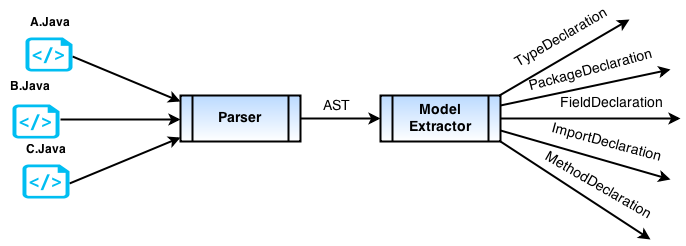
\includegraphics[width=0.98\textwidth]{Figures/parserINOut.png}
\caption{The Parser and Model Extractor components}
\label{fig:parserINOut}
\end{figure}

\subsection{Transformer}

The core of the tool suite is the Transformer. The Transformer receives a base language model (e.g. JavaModel, CPPModel OR PHPModel) from the extractor and an empty Umple model which is then populated. In fact, the base language model is decomposed into a series of objects representing each particular piece of the source code (a package, an import, a field and so on). Furthermore, the base-language model is transformed using a predefined set of mapping rules. If the input model is Umple code, the transformer produces an Umple model with additional modeling constructs (abstractions). The input/output relationship for the Transformer component is illustrated in Figure 
\ref{fig:transformerInOut}.

\begin{figure}[h]
\centering
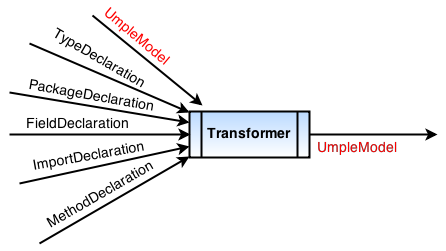
\includegraphics[width=0.70\textwidth]{Figures/transformerINOut.png}
\caption{The Transformer component inputs and outputs}
\label{fig:transformerInOut}
\end{figure}

As we have seen in Table \ref{table:technologies}, the Transformer component leverages Drools technologies to implement its rule engine.

\subsubsection{Drool's Rule Engine}

The rule engine interprets and executes the mapping rules on the source model and target model to produce the umplified version of the target model.
The Drools engine used by the Umplificator is composed of an inference engine that is able to scale to a large number of rules and facts.  The inference component matches facts and data (base language models) against rules to infer conclusions, which result in actions (model transformations). A rule is a two-part structure (Left-hand-side part and Right-hand-side part) using first order logic for reasoning over knowledge representation.

At a high level structural view, the Rule Engine consists of an: \textit{Inference Engine}, \textit{Agenda}, \textit{Pattern Matcher} and a \textit{Production} and \textit{Working Memory}. 
The rules are stored in the \textit{Production Memory} and the facts that the Inference Engine matches against are kept in the \textit{Working Memory}.
Facts are the data in which the rules act (Model elements in our case).
Pattern matching is performed to match facts against rules and is implemented using the Rete algorithm \cite{reteDROOLS}. Facts are evaluated into the Working Memory where they may be modified or retracted. The \textit{Agenda} manages the execution order of the rules. Figure \ref{fig:RuleEngineArchitecture} shows the difference components of the Rule Engine.

\begin{figure}[h]
\centering
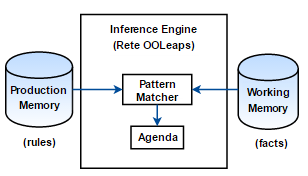
\includegraphics[width=0.75\textwidth]{Figures/RuleEngineArchitecture.png}
\caption{High Level View of the Drools Rule Engine}
\label{fig:RuleEngineArchitecture}
\end{figure}

Traditionally, rule engines have two methods of execution \cite{RulebasedSystems} forward chaining and backward chaining. In forward chaining, the facts are asserted into working memory resulting in one or more rules being concurrently true and scheduled for execution. In backward chaining (goal driven), one starts with a conclusion, which the engine tries to satisfy. Drools is a Hybrid Chaining System because it implements both forward and backward mechanisms. Our Umplificator uses the forward chaining method of operation in which the inference engine starts with facts, propagates through the rules, and produces a conclusion (e.g. a transformation). Figure \ref{fig:backwardForward} contrasts the two modes of execution. In Forward Chaining, the engine discovers what conclusions can be derived from the data and asserts them (iteratively), whereas in Backward chaining the engine starts with the goals and searches how to satisfy them (as in Prolog).

% Reference the figure number when you say 'figure below'
% MG FIXED
Consider the scenario of a model transformation in Figure \ref{fig:backwardForward}: if the conditions C1,C2 and C3 apply on a base language element, then we can perform the transformation as dictated bv D1. 
On the other hand, in backward chaining, we perform the transformation and then attempt to determine if it was correct based on the available information (C1,C2,C3 and input model element).

\begin{figure}[h]
\centering
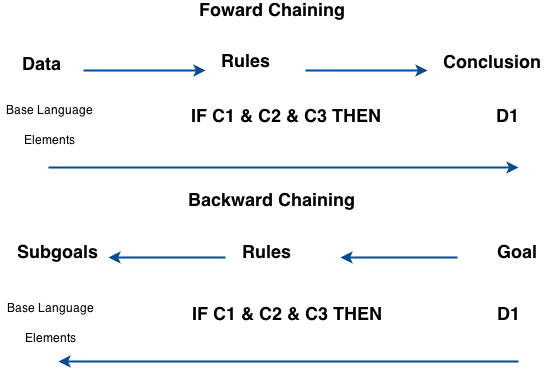
\includegraphics[width=0.80\textwidth]{Figures/ForwardBackwardChaining.png}
\caption{Forward vs Backward Chaining}
\label{fig:backwardForward}
\end{figure}

\subsubsection{The Rule Language}
The rule engine is initialized with the rules. Drools offers a native rule language, very light in terms of punctuation and supporting Java and domain specific languages. 

A rule file in Drools (and in our implementation) is a file with a .drl extension that can have the following elements:

\begin{itemize}
\item \textbf{Package}: The package name, if declared, must be the first element in the rule file and represents the namespace, which is kept unique for a given grouping of rules.
\item \textbf{Imports}: These are used to import Java types referenced by the rules.
\item \textbf{Global Variables:} A Global variable is a variable visible to all the rules inside a rule file. These are not inserted into the Working Memory and are most commonly used to log information on the execution of rules.
\item \textbf{Functions}: These are used for invoking actions on the consequence (then) part of the rule, especially if that particular action is used over and over again. 
\item \textbf{Queries}: These provide a means to search working memory and store the results under a named value. In the Umplificator, they are used to gather metric information about the models analyzed. For instance, the query  numberOfPublicMethods(..) returns the number of methods having `public' as modifier. Queries do not have side effects, meaning that their evaluation cannot alter the state of the corresponding executing unit. 
\end{itemize}

The rules as explained in this section are instructions indicating how a piece of the Base language model (Java Model, C++ model, etc.) is mapped to a piece of an Umple model. In the Umplificator, the logic used for model transformations resides in the rules. Moreover, by using rules, we have a single point of truth, a centralized repository of knowledge. Rules can be also read and understood easily, so they can also serve as documentation.

Listing \ref{lst:droolsrule} shows the basic form of a rule in Drools language, where LHS is the conditional part of the rule and RHS is a block that allows dialect-specific semantic code to be executed.  Attributes (Line 2) provides 
a declarative way to influence the behavior of the rule. We present the rule attributes used in our mapping rules in Table \ref{table:ruleattributes}.

% Refer to the listing number since a figure could get in the way
% MG FIXED
\begin{lstlisting}[language={drools},label={lst:droolsrule}, caption=Basic rule in Drools] 
rule "name" 
  attributes 
  when LHS then RHS
end
\end{lstlisting}

\begin{table}[h]
\caption{Rule attributes}
\label{table:ruleattributes}
\begin{tabularx}{\textwidth}{l|YY}
\toprule
\rowcolor[HTML]{BBDAFF}
\textbf{Attribute Name} & \textbf{Description}   \\ \hline	
\textbf{no loop} & Avoids infinite loops. When a rule's consequence modifies a fact it may cause the rule to activate again, causing an infinite loop; its default value is false.\\ \hline
\textbf{lock-on-active} &  Stronger version of no-loop. If a rule declares this attribute, the rule can be activated once.   \\ \hline
\textbf{Salience} & Salience is a form of priority where rules with higher salience values are given higher priority when ordered in the Activation queue; its default value is 0. \\ \hline
\textbf{agenda-group} & Agenda groups allow the user to partition the Agenda providing more execution control. Only rules in the agenda group that has acquired the focus are allowed to fire.     \\ \hline
\end{tabularx}
\end{table}

% At the start of this, say 'In Listinv X, LHS is the ...'
%MG FIXED
\textbf{Order of Execution and Grouping}

The rules are grouped in files for each of the cases (levels of refactoring) discussed earlier. In other words, there is a rule file containing rules, functions and queries to transform classes, namespace and imports; another file containing those to transform variables into attributes, another file containing those to transform variables into associations and so on.

To activate the groups on the required order, we used agenda groups. Agenda groups are a way to partition the activation. At any one time, only one group has `focus' meaning that activation for rules in that group will take effect. 
In other words, agenda groups provide a way to create a flow between grouped rules. They work as a stack. When we set the focus to a given agenda group, that group is placed on top of the stack. When the engine tries to fire the next activation and there are no more activations in a given group, that group is removed from the top of the stack and the group below receives focus again.

The Umplificator executes the rules to transform classes first, followed by the rules transforming attributes and finally by the rules transforming associations. 

We use the attribute agenda-group in the rules to specify the order of the activation. For instance, the rule in Listing \ref{lst:agendagroup} is a rule belonging to the group that will be executed first. The rule in Listing \ref{lst:agendagroup2} will be executed after any rule belonging to the first level. 

\begin{lstlisting}[language={drools},label={lst:agendagroup}, caption=A rule belonging to Level 1] 
rule "transform_Namespace_UInterface"
	agenda-group "LEVEL1" 
	when
	// parts omitted
	then
	// parts omitted
end
\end{lstlisting}

\begin{lstlisting}[language={drools},label={lst:agendagroup2}, caption=A rule belonging to Level 2] 
rule "JavaField_CanBeUmpleAttribute"
	agenda-group "LEVEL2" 
	when
	// parts omitted
	then
	// parts omitted
end
\end{lstlisting}

Listing \ref{lst:fireAllRules} shows how the rules are inserted into the Working Memory of the Umplificator rule engine. Level 3 will be put on the bottom of the stack, followed by Level 2 rules, and Level 1 rules which will be on the top of the stack. The \textit{KieSession} object represents the working memory of the Rule Engine.

\begin{lstlisting}[style=java, caption=Firing the rules in the Umplificator, label=lst:fireAllRules]
public KieSession fireAllRules()
{
// Agenda works as a stack
kieSession.getAgenda().getAgendaGroup( "LEVEL3" ).setFocus();
kieSession.getAgenda().getAgendaGroup( "LEVEL2" ).setFocus();
kieSession.getAgenda().getAgendaGroup( "LEVEL1" ).setFocus();
kieSession.fireAllRules();

return kieSession;
}
\end{lstlisting}

More details on the different mapping rules will be presented in Section \ref{sec:automatedUmplification}.

\subsection{Generator}

The Generator component validates the received UmpleModel and generates Umple code from it. That is, it generates an Umple file for each class or interface in the Umple model.

\begin{figure}[h]
\centering
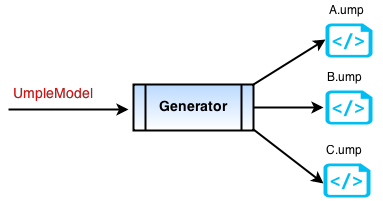
\includegraphics[width=0.55\textwidth]{Figures/generatorINOut.png}
\caption{The Generator component inputs and outputs}
\label{fig:generatorInOut}
\end{figure}

The Generate supports different options when it comes to generation of output files.  One way to do this is to follow the Java convention of having one .ump file per class. Another common approach is to have one or more files for the model code (just the pure UML elements such as classes with their attributes, associations and state machines) and separate files for the methods; we can in fact have some files for Java methods, and other files for PHP or Ruby methods. The same model can then be used to develop systems that are deployed in multiple base languages. For instance, for the Java  input class\textit{A.java}, the two following files would be generated:

\begin{enumerate}
\item \textit{A.ump}: containing methods, algorithmic and logic code for class A.
\item \textit{A\_model.ump}: Modeling constructs for class A.
\end{enumerate}

The Generator supports also the creation of directories to preserve the namespace structure. For instance, if the namespace of the Umple file is `cruise.Umple', the Generator will create two directories, `cruise' and `Umple' (inside).

\section{Automated Umplification Example}
\label{sec:automatedUmplification}
\subsection{Initial transformation}

As an example of the transformation process using the Umplificator, consider the input Java source code in Listing \ref{lst:exampleTransformer}.
We want to achieve the initial level of refactoring (Level 1).

\begin{lstlisting}[style=java, caption=Input source code, label=lst:exampleTransformer]
package university;

import java.util.Date;

public class Student {
	
    private String name;
    private int studentId;
    
    public Student (int studentId) {
    	this.studentId = studentId;
    }
    public String getName () { return name;}
    
    public void  setName (String aName) { 
    	this.name =  aName;
    }
   
    public int getStudentId () { return studentId;}
    
    public String toString() {
    	return "The student " + name "has id=" + studentId;
    }
}   
\end{lstlisting}

The \textit{Parser} receives the source code above, creates an Abstract Syntax Tree representation of it and transfers it to the Model Extractor. The Model Extractor uses the AST representation to create a Java model which is then traversed and decomposed in pieces by means of a Java class visitor. Table \ref{table:exampleTransformer} presents all the Java Elements collected by the Java visitor.

\begin{table}[h]
\caption{The input Java Model elements}
\label{table:exampleTransformer}
\begin{tabularx}{\textwidth}{l|l}
\toprule
\rowcolor[HTML]{BBDAFF}
\textbf{ASTNode Type} & \textbf{Source Fragment}  \\ \hline	
\textbf{PackageDeclaration} & "package university;" \\ \hline
\textbf{ImportDeclaration} & "import java.util.Date;" \\ \hline
\textbf{TypeDeclaration} &  "public class Student"  \\ \hline
\MyIndent \textbf{FieldDeclaration} &  "public String name;"  \\ \hline
\MyIndent \textbf{FieldDeclaration} &   "public int studentId;"  \\ \hline
\MyIndent \textbf{MethodDeclaration} &  "public int getStudentId () {...}"  \\ \hline
\MyIndent \textbf{MethodDeclaration} &  "public String getName () {...}"  \\ \hline
\MyIndent \textbf{MethodDeclaration} &  "public void  setName(...) {}"  \\ \hline
\MyIndent \textbf{MethodDeclaration} &  "public Student(...){}"  \\ \hline
\MyIndent \textbf{MethodDeclaration} &  "public String toString(){...}"  \\ \hline
\end{tabularx}
\end{table}

The Transformer receives the Java model elements in Table above, together with a newly created instance of an UmpleModel and places them into the Working Memory.  At this point of time, the \textit{Production Memory} contains all rules  but the \textit{Agenda} contains only those belonging to this level of refactoring (those with attribute `agenda-group LEVEL1'). 

% You refer to Table above when you need to refer to it by name

When the model elements (facts) are inserted into the memory, the pattern matching begins. The rule engine then tries to find objects matching the conditions in the rules. The only rule meeting all the conditions and that can be matched to objects in the Working Memory is the rule named \textit{addClassToUmpleModel}. The rule is presented in Listing \ref{lst:addClassToUmpleModel}.

\begin{lstlisting}[language={drools},label={lst:addClassToUmpleModel}, caption=Rule 'addClassToUmpleModel']
rule "addClassToUmpleModel"
 agenda-group "LEVEL1" 
 when
  typeDeclaration: TypeDeclaration()
  umpleModel: UmpleModel()
 then
  String typeName = getTypeDeclarationName(typeDeclaration);
  UmpleClass umpleClass = new UmpleClass(typeName);
  umpleModel.addUmpleClass(umpleClass);
  insert(umpleClass);
end
\end{lstlisting}

The rule above simply requires the presence in the Working Memory of an instance of TypeDeclaration (Line 4) and an instance of an UmpleModel (Line 5). As the conditions are satisfied, in the RHS of this rule we create a new instance of UmpleClass, setting its name. To extract the name of the instance \textit{TypeDeclaration} we employ a helper function \textit{getTypeDeclarationName(...)}. After the object is created, we insert it into the session with the `\textit{insert(umpleClass)}' method. This process of matching facts with rules (i.e. inference) is illustrated in Figure \ref{fig:ruleModel}.

\begin{figure}[h]
\centering
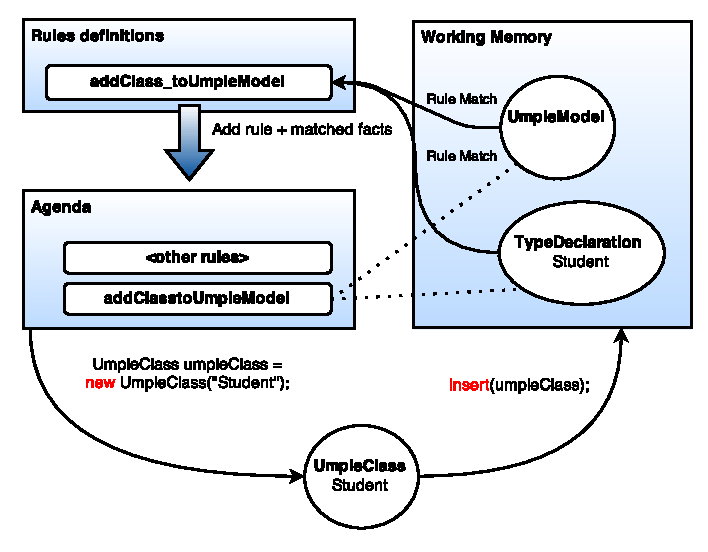
\includegraphics[width=0.98\textwidth]{Figures/ruleModel.pdf}
\caption{Pattern Matching and creation of an UmpleClass}
\label{fig:ruleModel}
\end{figure}

After the insertion of the UmpleClass into the working memory, the inserted object can generate more rule matches. The UmpleModel residing in the Working Memory now contains one Umple class. It is automatically updated by the engine.

The rules for the remaining Umple class constructs are then matched. The goal of these rules is to populate the Umple class based on the information obtained from the typeDeclaration. 

The rule named \textit{transformImportDeclaration} (Lines 1-11) in Listing \ref{lst:ruleImport} matches and converts any Import Declaration (Java Language) into an Umple depend construct. The dependency (Line 9) is then added to a matched Umple Class. The Umple Class residing in the Working Memory is then updated at Line 10.

To ensure that the dependency is not added to any umpleClass in the Working Memory but only to the one owning it, we assert that the ImportDeclaration's parent class has the same name as our targeted UmpleClass. The helper function, imported in the first line of the above Listing, is a static function that returns the name of the parent class of the ImportDeclaration. In our case, the name of parent Java class is ``Student'' which corresponds to the name of a UmpleClass in memory. The `eval' clause returns true in this particular case.

\begin{lstlisting}[language={drools},label={lst:ruleImport}, caption=Rule transformImportDeclaration]
import function cruise.umplificator.rules
       .TopLevelAnalyzerHelper.getDeclarationContainerName
      
rule "transformImportDeclaration"
 agenda-group "LEVEL1" 
 when
  importDeclaration: ImportDeclaration()
  uClass: UmpleClass()
  eval(uClass.getName()
       .equals(getDeclarationContainerName(importDeclaration)))		
 then
  Depend depend = new Depend(getImportName(importDeclaration));
  uClass.addDepend(depend);
  update(uClass);
 end
\end{lstlisting}

The package declaration is converted then into a namespace with the rule `transformNamespace' in Listing \ref{lst:transformNamespace}. We again ensure that the package declaration corresponds to the targeted UmpleClass. Note that in this rule we don't need to insert the namespace object into memory since we don't expect any rule to match it.

\begin{lstlisting}[language={drools},label={lst:transformNamespace}, caption=Rule transformNamespace]
import function cruise.umplificator.rules
       .TopLevelAnalyzerHelper.getDeclarationContainerName
rule "transform_Namespace"
 agenda-group "LEVEL1" 
 when
  packageDeclaration: PackageDeclaration()
  uClass: UmpleClass()
  eval(uClass.getName()
      .equals(getDeclarationContainerName(packageDeclaration)))	
 then
  uClass.addNamespace(packageDeclaration.getName()
                      .getFullyQualifiedName());
end
\end{lstlisting}

As we have assumed an initial level of refactoring. at the beginning of this example, the Transformer will not attempt to transform any variable into an Umple attribute, association end or state machine. However, in the final output code produced for our UmpleClass we require the remaining untreated code to be simply appended. For instance, the rule `appendFieldDeclaration' in Listing \ref{lst:appendField} extracts information from the field declaration and appends it to the targeted Umple Class. The same behavior is produced from the application of rule `appendMethodDeclaration' in Listing \ref{lst:appendMethod}.

\begin{lstlisting}[language={drools},label={lst:appendField}, caption=Rule appendFieldDeclaration]
import function cruise.umplificator.rules
       .TopLevelAnalyzerHelper.getDeclarationContainerName
       
rule "appendFieldDeclaration"
 agenda-group "LEVEL1" 
 when
  fieldDeclaration: FieldDeclaration()
  uClass: UmpleClass()
  eval(uClass.getName()
       .equals(getDeclarationContainerName(fieldDeclaration)))
  eval(!uClass.getExtraCode().contains(fieldDeclaration.toString()))
 then
  uClass.appendExtraCode(fieldDeclaration.toString());
  update(uClass);
end
\end{lstlisting}

The \textit{eval} clauses in the Listing above, ensure that the string representing the field information hasn't been appended before and (as before) that the field string is added to the Umple class owning it.

% instead of saying 'Listing above' refer to the listing by number

\begin{lstlisting}[language={drools},label={lst:appendMethod}, caption=Rule appendMethodDeclaration]
import function cruise.umplificator.rules
       .TopLevelAnalyzerHelper.getDeclarationContainerName
       
rule "appendMethodDeclaration"
 agenda-group "LEVEL1" 
 when
  method: MethodDeclaration()
  uClass: UmpleClass()
  eval(uClass.getName().equals(getDeclarationContainerName(method)))
  eval(!uClass.getExtraCode().contains(method.toString()))
 then
  uClass.appendExtraCode(method.toString());
  update(uClass);
end
\end{lstlisting}

The \textit{eval} clauses in the Listing above, ensure that the string representing the method information hasn't been appended before and (as before) that the method string is added to the Umple class owning it. 
At the end of this pattern matching process, the UmpleClass with name `Student' owns a depend, has a namespace and some remaining code that we called extra code. We show the Umple code in Listing \ref{lst:level1exampleGenerator}. The extra code in this code excerpt starts from Line 6 to 22.

The code generated by the \textit{Generator}, from the input Umple model, is presented in Listing \ref{lst:level1exampleGenerator}. 

This concludes the initial transformation step.

\begin{lstlisting}[style=umpleOut, label=lst:level1exampleGenerator, caption=Umple code generated -- Level 1]
namespace university.student;

class Student {
	depend java.util.Date;
	
    public String name;
    public int studentId;
    
    public Student (int studentId) {
    	this.studentId = studentId;
    }
    public String getName () { return name;}
    
    public void  setName (String aName) { 
    	this.name =  aName;
    }
   
    public int getStudentId () { return studentId;}

    public String toString() {
    	return "The student " + getName() "has id=" + getStudentId();
    }
}   
\end{lstlisting}

\subsection{Automated Umplification of Attributes}

As an example of the pattern matching for rules in Level 2 (attributes), consider the same code excerpt from Listing \ref{lst:exampleTransformer}. The process described in the previous example remains identical, except for the transformations phase, which we explain now. Assuming that the rules for the transformation of the package and import declarations have already been performed, we focus exclusively on how the field declarations are transformed into Umple attributes. In this particular example we are expecting the two Java field declarations to be transformed into attributes. 

At this point of time, as illustrated in Figure \ref{fig:ruleModel2}, the Working Memory contains the Umple model, an Umple Class (Student) and the Java model elements. The Production Memory contains all the `LEVEL1' and `LEVEL2' rules and the Agenda only those from `LEVEL2' since the ones from `LEVEL1' have already been executed and removed from the stack.

\begin{figure}[h]
\centering
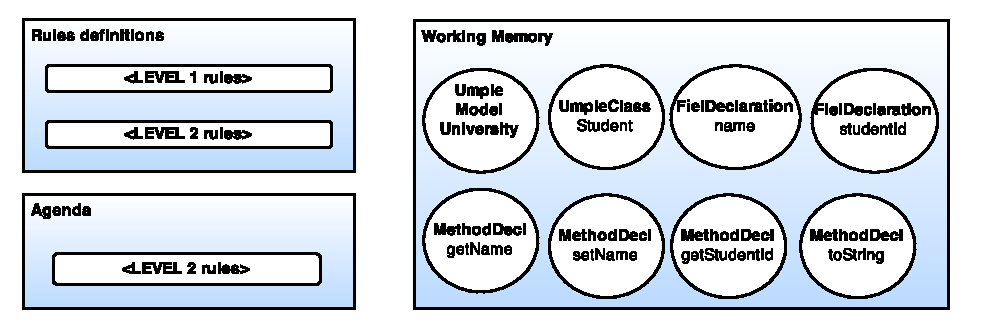
\includegraphics[width=0.98\textwidth]{Figures/ruleModel2.pdf}
\caption{Rule Engine snapshot after initial transformation}
\label{fig:ruleModel2}
\end{figure}

The rule engine then attempts to find objects matching the conditions in the rules. The only set of rules that can be matched to objects in the Working Memory are the rules related to attributes since the only rules in the agenda are those for 'LEVEL2' and the rules for `LEVEL1' have already been applied. In particular, the unique rule
that can be executed at this moment is the rule named \textit{`Field\_CanBeUmpleAttribute'} since all other rules require an instance of an Umple attribute in memory. As we have illustrated before in Figure \ref{fig:ruleModel2}, no instances of an Umple attribute exist or have been added so far. Rule \textit{`Field\_CanBeUmpleAttribute'} is presented in Listing \ref{lst:FieldCanBeUmpleAttribute}.

\begin{lstlisting}[language={drools},label=lst:FieldCanBeUmpleAttribute, caption=Rule  FieldCanBeUmpleAttribute]
rule "FieldCanBeUmpleAttribute"
agenda-group "LEVEL2" 
 when
	fieldDeclaration: FieldDeclaration()
	uClass: UmpleClass()
	method: MethodDeclaration()
	eval(isPrimitiveOrStringOrTime(fieldDeclaration))				   
	eval(uClass.getName()
	     .equals(getFieldCuATTontainerName(fieldDeclaration)))
	eval(uClass.getName().equals(getMethodContainerName(method)))
	eval(uClass.getAttribute(getFieldName(fieldDeclaration))== null)
	eval(hasFieldAGetter(method, fieldDeclaration, uClass.getName()))
 then 
	String attrName = getFieldName(fieldDeclaration);
	String attrType  = getAttributeType(fieldDeclaration);
	Attribute uAttr = 
	  new Attribute(attrName, attrType, null, null, false, uClass);
	uAttr.setModifier("settable");
	uClass.addAttribute(uAttr);
	removeClassField(fieldDeclaration, uClass);
	update(uClass);    	
	insert(uAttr);
end
\end{lstlisting}

The rule in Listing \ref{lst:FieldCanBeUmpleAttribute} creates an Umple attribute with information extracted from a field declaration. It does so indeed, only if the following conditions are met:
\begin{itemize}
\item In Lines 4,5,6. We require instances of a field, Umple class and method declarations in order to assess whether or not the field can become an Umple attribute. These elements need to be found in the Working Memory. 
\item In Line 7. The field needs to be of a primitive type.
\item In Line 8-9. The field needs to be declared in the Class that derived the current instance of the Umple Class.
\item In Line 10. The method declaration needs to be declared in the Class that derived the current instance of the Umple Class.
\item In Line 11. The Umple class must not possess an attribute with the name of the current instance of the field declaration. This is to avoid duplicates.
\item In Line 12. The field possess a getter in the Class that derived the current instance of the the Umple Class.
\end{itemize}

If a field (and other model elements) matches the above conditions. A new Umple attribute is created with the information extracted from the instance of the field declaration and associate to the current instance of Umple Class (Line 16). The name (Line 14) and type (Line 15) are initialized as well. By default, our newly created Umple attribute is declared as settable (Line 17). The attribute is then added to a matched Umple Class (Line 18). The Helper function \textit{removeClassField} in Line 18 removes the field declaration from the extra code of the Umple Class since it has been refactored into an Umple attribute. Recall from previous subsection that the field declaration was appended to the extra code of the Umple class. In Line 19, we updated the Umple class residing in the Working Memory. The clause `\textit{update}' is optional but we explicitly invoke it for logging purposes.

Finally, in Line 20 the attribute is put into the working memory so subsequent transformations can be made such as determining if the attribute is lazy or not. In fact, this Umple attribute as we will explain later, meets all conditions to be a `lazy' attribute. Lazy attributes have been introduced in Chapter 2. This process of matching objects with rules as we have described so far for this transformation step is summarized in Figure \ref{fig:ruleModel3}. As can be seen in the Figure, an instance of a the Umple attribute has been added to the Working Memory as a result of the match. Objects in yellow are the ones queried when evaluating the conditions of the rule. 

\begin{figure}[h]
\centering
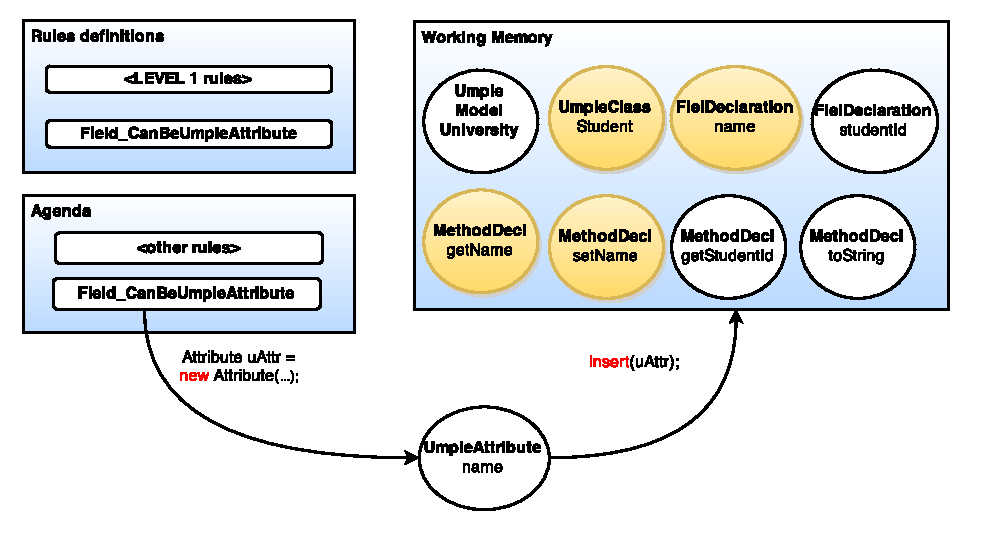
\includegraphics[width=0.98\textwidth]{Figures/ruleModel3.pdf}
\caption{Pattern Matching and creation of an UmpleClass}
\label{fig:ruleModel3}
\end{figure}

We are not done yet since we need to remove or refactor the getters  and/or setters of the field (that became an attribute). For instance, if the rule (omitted) `\textit{hasFieldSimpleGetter}' or `\textit{hasFieldSimpleSetter}' is matched to any field previously transformed into an attribute, the method declaration is removed from the appended code of the Umple class. As is the case in our example, getName(), setName() and getStudentId() are removed from the `Student' Umple class.
When the field has a getter/setter that is not simple, an instance of the class CodeInjection (refer to Umple metamodel) is created to take into account the code differing from the original getter/setter.

Finally, the rule named \textit{isLazyAttribute} in Listing \ref{lst:isLazyAttribute},  rule matches and converts any basic attribute (in memory) that conforms to the required conditions into a lazy attribute (e.g. attribute.setIsLazy(true)). These required conditions are listed next (Lines refer to Listing \ref{lst:isLazyAttribute}): 

\begin{itemize} 
\item In Lines 4,5,6. We require instances of a field, Umple class, method declaration and an Umple attribute in order to assess whether or not the attribute can become a lazy attribute. These elements need to be found in the Working Memory. 
\item In Line 8. The current instance of the Umple class needs to be the one owning the Umple attribute.
\item In Line 9. The field needs to be declared in the Class that derived the current instance of the Umple Class.
\item In Line 10. The method declaration needs to be declared in the Class that derived the current instance of the Umple Class.
\item In Line 11. A (double) check to ensure that the attribute belongs to the class.
\item In Line 12. The current instance of the field declaration is the one used to derived the current instance of the attribute.
\item In Line 13: The class in which the field is declared is NOT one of the constructor arguments. As per definition of a lazy attribute.
\end{itemize}

\begin{lstlisting}[language={drools},label=lst:isLazyAttribute, caption=Rule isLazyAttribute]
rule "isLazyAttribute"
agenda-group "LEVEL2" 
 salience 50
 when
  fieldDeclaration: FieldDeclaration()
  method: MethodDeclaration(method.isConstructor())
  attribute: Attribute(isLazy==false)
  uClass: UmpleClass(getAttributes().size() > 0 && 							      getAttributes().contains(attribute))
  eval(uClass.getName().equals(getFieldContainerName(fieldDeclaration)))
  eval(uClass.getName().equals(getMethodContainerName(method)))
  eval( attribute.getUmpleClass() == uClass) 
  eval( attribute.getName().equals(getFieldName(fieldDeclaration))) 
  eval(isFieldInContructor(method, fieldDeclaration, uClass.getName())==false);
  eval(getFieldName(fieldDeclaration).equals(attribute.getName()));
 then
  attribute.setIsLazy(true);
  update(attribute);
end
\end{lstlisting}

Since there are no more rules to execute, the rule engine stops. The update Umple model is passed to the Generator for code generation. Note that the method \textit{toString()} is still part of the extra code of the Student Umple class.
The code generated by the \textit{Generator}, from the populated Umple model, is presented in Listing \ref{lst:level2exampleGenerator}. This concludes our second transformation step.

\begin{lstlisting}[style=umpleOut, label=lst:level2exampleGenerator, caption=Umple code generated -- Level 2]
namespace university.student;

class Student {
 depend java.util.Date;
	
 lazy String name;
 Integer studentId;
       
 public String toString() {
  return "The student " + getName() "has id=" + getStudentId();
 }
}   
\end{lstlisting}

In this next section, we provide an overview of the tools currently available to support the umplification reverse-engineering process.

\section{Umplificator Tooling}

The Umplificator is available as an IDE and works within Eclipse; it also operates as a command-line tool to allow rapid bulk umplification and easier automated testing. Both tools are built and deployed using the Ant scripting language; resulting in several executable jars as well as for the Eclipse plugins. Table \ref{table:jars} describes the various jars deployed as part of our automated building process. In the table, X corresponds to the version, Y to the revision and Z to the build number. Our current version is `1.21.0.4666'.

\begin{table}[h]
\caption{Artifacts deployed during the building process of the Umplificator}
\label{table:jars}
\begin{tabularx}{\textwidth}{l|Y}
\toprule
\rowcolor[HTML]{BBDAFF}
\textbf{Name} & \textbf{Description}  \\ \hline	
cruise.umplificaror.eclipse\_vX.X.X.jar &  Plug-in for the Eclipse IDE 
\\ \hline
umplificator\_X.Y.Z.jar & Command-Line tool for umplification 
\\ \hline
validator\_X.Y.Z.jar & Command-Line tool that checks whether the input Umple code generates compilable base language code. 
\\ \hline
\end{tabularx}
\end{table}

Umplifying source code by means of the command-line tool can be done using the following command:

\vspace{\baselineskip}
\begin{lstlisting}[style=umplePlain]
< java -jar umplificator_1.21.0.4666.jar inputFile -level=1,2,3 
       -splitModel -dir -path >
\end{lstlisting}

where:
\begin{itemize}
\item \textbf{inputFile} can be an Umple file, base language file (.java, .cpp) or Source directory (containing java/Umple/cpp files).
\item \textbf{level}: can be 0,1,2 and corresponds to the refactoring that wants to be achieved. 0 for the initial (classes, namespace, imports, etc.); 1 for the refactoring of attributes; 2 for the refactoring of associations. Level 2 includes transformations from level 0 and 1. Level 1 includes (and requires) transformations from level 0.
\item \textbf{splitModel} (optional): creates two files for each input file; one containing the modeling constructs, one containing the algorithmic and logic code (extra code). 
\item \textbf{dir} (optional): creates directories following the namespace structure.
\item \textbf{path}: the output directory name where the resulting Umple files will be located.
\end{itemize}

Additionally, the Umplificator is available as an online tool, called UmplificatorOnline. The tool is under development but will be deployed soon for public access. We have created this project for several purposes. Casual users are able to experiment with the latest version of the Umplificator with no more than a browser and an Internet connection. This allows curious developers to try out the tool. Figure \ref{fig:umpleonline} presents the initial page of the UmplificatorOnline.
An open-source project \textit{downloader} has been implemented as part of this Web tool. Please note that the tool runs the  Umplificator main jar (umplificator\_1.21.0.4666.jar) for its reverse engineering capabilities. 

The preliminary release of the tool allows developers to:

\begin{itemize}
\item Select and Open-Source \textbf{repository}: User can select projects from GoogleCode, SourceForge or GitHub.
\item Select an Open-Source \textbf{project} to umplify. The projects listed (in the second combo-box) have been automatically selected based on a number predefined criteria. The criteria for project selection are that project is marked as small or medium-size system and that the project is written in Java or C++.
\item Select the \textbf{level} of refactoring desired.
\item Select one of more \textbf{options}. The options have been described during our discussion on the command-line tool.
\end{itemize}

\begin{figure}[h]
\centering
\frame{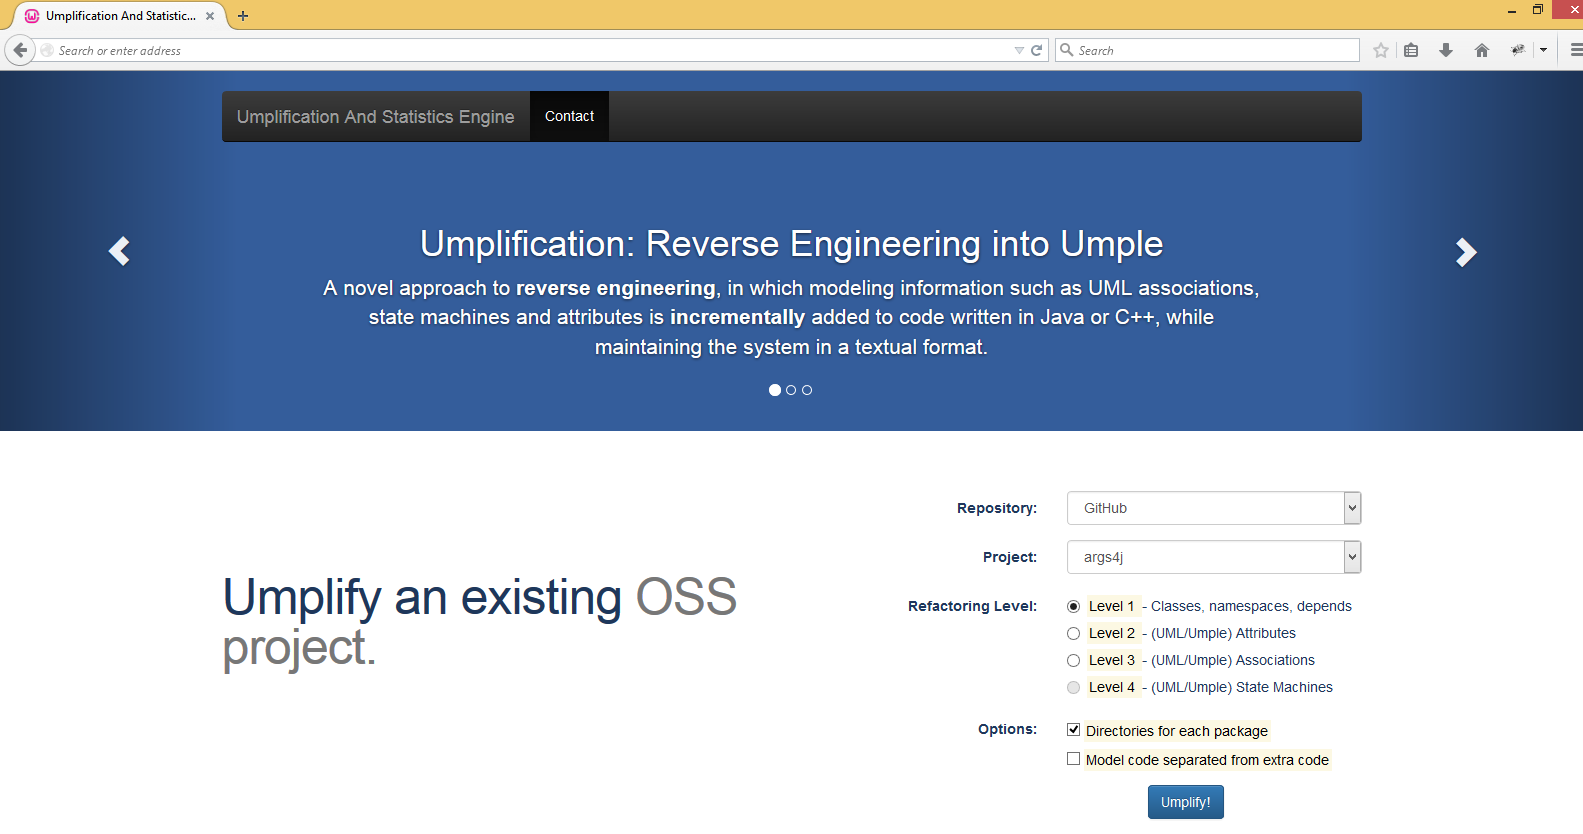
\includegraphics[width=0.98\textwidth]{Figures/UmplificatorOnline.png}}
\caption{The Umplificator online - A PHP Web application}
\label{fig:umpleonline}
\end{figure}


